\documentclass[final,5p,times,twocolumn,authoryear]{elsarticle}

\usepackage{amssymb}
\usepackage{lipsum}
\usepackage{amsthm}
\usepackage{amsmath}
\usepackage[utf8]{inputenc}
\usepackage{lineno}

%% You might want to define your own abbreviated commands for common used terms, e.g.:
\newcommand{\pd}[2]{\frac{\partial #1}{\partial #2}}
\newcommand{\pdd}[2]{\frac{\partial^2 #1}{\partial #2^2}}

\journal{Graduate School@UGA}

\begin{document}

\begin{frontmatter}

%% Title, authors and addresses

\title{Simulations of stratified turbulence and comparison with oceanic wave turbulence}

\author[first]{Guillermin Remy}

\begin{abstract}
%% Text of abstract

\end{abstract}

%%Graphical abstract
%\begin{graphicalabstract}
%\includegraphics{grabs}
%\end{graphicalabstract}

%%Research highlights
%\begin{highlights}
%\item Research highlight 1
%\item Research highlight 2
%\end{highlights}

\begin{keyword}
%% keywords here, in the form: keyword \sep keyword, up to a maximum of 6 keywords
Numerical Simulation \sep Fluids Dynamic \sep Turbulence

%% PACS codes here, in the form: \PACS code \sep code

%% MSC codes here, in the form: \MSC code \sep code
%% or \MSC[2008] code \sep code (2000 is the default)

\end{keyword}


\end{frontmatter}

%\tableofcontents

%% \linenumbers

%% main text

\section{Introduction}
\label{introduction}

In fluid mechanics, turbulence arises when the Reynolds number, $\mathrm{Re} = UL/\nu \gg 1$, where $U$ and $L$ are the characteristic velocity and length scales of the flow, and $\nu$ is the kinematic viscosity. This condition is typically met in scenarios such as high-speed flows (e.g., jet engine exhaust), large-scale flows (e.g., atmospheric or ocean currents), or in fluids with negligible viscosity, like superfluids. Turbulence is characterised by chaotic, irregular motion that significantly affects the transport of momentum, heat, and mass.

In the context of large-scale climate systems, such as the ocean and atmosphere, turbulence is even more complex due to the additional influence of Earth’s rotation and the stratification of the fluid—either by temperature (in the atmosphere) or density (in the ocean). These factors modify the basic dynamics described by the Navier-Stokes equations. Specifically, stratification leads to the formation of internal waves, which in turn interact with turbulence in intricate ways, driving the transport and mixing processes that are fundamental to climate dynamics.

This project focuses on the effects of density stratification in large-scale flows, particularly how it induces internal wave turbulence. Understanding this phenomenon is crucial because internal waves play a key role in energy transfer within oceans and atmospheres, influencing ocean currents and atmospheric circulation patterns. By studying turbulent flows under stratified conditions, we aim to gain insights into the mechanisms governing large-scale climate dynamics and the energy cascades that drive these systems.


\section{Theoretical background}
\subsection{Navier-Stokes Equations}

The governing equations for fluid motion in this study are the Navier-Stokes equations, given by:
\begin{subequations}
\begin{align}
\pd{\rho}{t} + \vec{\nabla} \left( \rho \vec{u} \right) &= 0 \\
\rho \left( \pd{\vec{u}}{t} + \left( \vec{u} \cdot \vec{\nabla} \right) \vec{u} \right) &= - \vec{\nabla} p - \rho g \hat{z} + \mu \Delta \vec{u}
\end{align}
\label{eq:NS}
\end{subequations}
where $\rho$ is the fluid density, $\vec{u}$ is the velocity field, $p$ is the pressure, $\mu$ is the dynamic viscosity, and $g$ is the acceleration due to gravity. These equations describe the motion of a viscous fluid, accounting for both inertial and gravitational forces.

\subsection{Dimensionless Numbers}

In the study of fluid mechanics, the Froude number $\mathrm{Fr}^2 = U^2 / gH$ is a key dimensionless quantity that represents the ratio of inertial forces (advection) to gravitational forces. Here, $U$ is the characteristic velocity, $g$ is gravitational acceleration, and $H$ is the characteristic depth or length scale of the flow. The Froude number is useful in understanding the behavior of stratified fluids, where gravity plays a significant role in the dynamics.

\subsection{Boussinesq Approximation and Wave Propagation}

For density stratified fluids, the Boussinesq approximation [\cite{boussinesq_theorie_1897}] is commonly applied, which assumes that density variations are small and only affect the buoyancy force, while the density is constant elsewhere. After applying this approximation to the Navier-Stokes equations and simplifying, we derive the wave propagation equation:
\begin{equation}
\partial^2_t \vec{u} = \left( N^2 \nabla^2_h \nabla^{-2} \right) \vec{u} \label{eq:Wave Propagation}
\end{equation}
where $\nabla_h$ is the horizontal gradient operator, $\nabla$ is the spatial gradient operator, and $N^2 = -\frac{g}{\rho} \pd{\rho}{z}$ is the Brunt-Väisälä frequency [\cite{pedlosky_geophysical_1979}]. This equation describes the propagation of internal waves in a stratified fluid.

\subsection{Dispersion Relation of Gravity Waves}

The dispersion relation for gravity waves, derived from the wave propagation equation, is given by:
\begin{equation}
\omega = \pm N \sin{\theta} \label{eq:Dispersion relation}
\end{equation}
where $\omega$ is the frequency of the wave, and $\theta$ is the angle between the wave-vector $\vec{k}$ and the vertical $z$-axis. This relation shows that the frequency $\omega$ is bounded within the range $\left[ -N, +N \right]$, where $N$ is the Brunt-Väisälä frequency, which determines the stability of stratified fluid systems.

\subsection{Poloidal-Toroidal Decomposition}

In incompressible flows, where $\vec{\nabla} \cdot \vec{u} = 0$, the velocity field can be decomposed into poloidal and toroidal components. The poloidal-toroidal decomposition [\cite{schmitt_decomposition_1992}] helps in analyzing the structure of turbulent flows in the vertical direction. The total kinetic energy $E_k$ can be written as the sum of the poloidal and toroidal components:
\begin{equation*}
E_k = E_p + E_t
\end{equation*}
where the specific kinetic energy of each component is given by:
\begin{equation*}
E_{p,t} = \frac{1}{2} \int_{\mathbb{R}^3} \left( \vec{u}_{p,t} \right)^2 d^3 \vec{r}
\end{equation*}
This decomposition helps isolate the different types of motion in the flow and is particularly useful when studying turbulence in stratified fluids.

\subsection{Potential Energy in Stratified Fluids}

The potential energy in a stratified fluid is related to density perturbations within the background stratification. It can be expressed as:
\begin{equation}
E_\phi = \left\langle \frac{g^2 {\delta \rho}^2}{2 N^2 \rho_0^{;2}} \right\rangle \label{eq:Potential Energy}
\end{equation}
where $\rho_0$ is the mean density of the fluid, and $\delta \rho$ represents the density perturbation from the mean value. This expression describes the potential energy associated with internal waves and density fluctuations in the fluid.

\section{Numerical Setup}

\subsection{Computational Tools}

For this study, we will use Fluidsim [\cite{fluiddyn}], a High-Performance Computing (HPC) code that utilises pseudo-spectral solvers. Fluidsim is well-suited for simulating fluid dynamics in stratified flows, providing efficient solutions for large-scale computations.



\subsection{Computational Environment}
We will perform simulations on three different platforms: a personal computer for small grid tests, a supercomputer named Zen hosted by Mesonet for larger-scale simulations, and the GRICAD cluster. Zen offers significant computational power for large simulations but does not provide the same parallelisation capabilities as the GRICAD cluster. Due to current issues with parallelisation on GRICAD, it is currently more efficient to alternate between Zen and GRICAD, depending on the specific parallelisation challenges encountered. Once the parallelisation issues on GRICAD are resolved, we plan to utilise its full parallel processing capabilities for even larger simulations.

\section{Simulation Parameters}
\subsection{Direct Numerical Simulation (DNS) Requirements}

We aim to perform Direct Numerical Simulations (DNS), which requires a high grid resolution that is smaller than the Kolmogorov length scale $\eta$. This ensures that all turbulence scales are resolved, providing accurate results for the flow dynamics. In DNS, we seek to capture the full range of turbulent scales from the large eddies down to the smallest dissipative structures.

\subsection{Reynolds Number and Kolmogorov Length Scale}

To resolve the smallest turbulent scales, we must ensure that the grid resolution is fine enough by selecting an appropriate Reynolds number $Re$. For Direct Numerical Simulations (DNS), the condition $k_{\text{max}} \eta > 1$ must be satisfied, where $k_{\text{max}}$ is the maximum wavenumber and $\eta$ is the Kolmogorov length scale. The largest wavenumber is given by:

\begin{equation*}
k_{\text{max}} = \frac{2\pi}{L_z} \frac{n_z}{2}
\end{equation*}

where $n_z$ is the number of grid points along the vertical spatial dimension and $L$ is the domain size. To satisfy the DNS condition, we require a relationship between $Re$ and $n_z$. The Kolmogorov length scale $\eta$ is related to the Reynolds number by the expression $\frac{L}{\eta} = Re^{3/4}$.

By equating the two conditions, we can express the Reynolds number as a function of the grid resolution parameter $n_x$:

\begin{equation}
Re < \left( \pi n_z \right)^{4/3}
\end{equation}

This ensures that the grid resolution is fine enough to resolve the smallest turbulent scales, satisfying the DNS requirements.

\subsection{Injection Rate and Richardson Number}

In our simulations, we do not directly control the velocity field but can adjust the energy injection rate $\varepsilon_i$. This injection rate is related to the characteristic velocity $U_i$ at the injection scale $l_i$ through the following relationship:

\begin{equation*}
U_i = (\varepsilon_i l_i)^{1/3}
\end{equation*}

It is important to note that the energy injection rate $\varepsilon_i$ at the injection scale is equal to the energy dissipation rate $\varepsilon_d$ at the dissipation scale. Therefore, we denote the constant energy transfer rate across scales as $\varepsilon$.

The Richardson number $Ri$ is a key parameter that characterizes the ratio of buoyancy forces to flow shear forces [\cite{cushman-roisin_introduction_2011}]. This dimensionless number is defined as:

\begin{equation}
Ri = \frac{N^2}{\left(d \bar{u} / dz \right)^2}
\end{equation}

where $N$ is the Brunt-Väisälä frequency, and $d\bar{u}/dz$ represents the vertical shear of the horizontal velocity. In our simulations, $Ri$ is a controllable parameter, enabling us to study the influence of stratification on the flow.

Using the Richardson number and the energy transfer rate, we can express the kinematic viscosity $\nu$ as:

\begin{equation*}
\nu = \frac{\varepsilon}{Ri \cdot N^2}
\end{equation*}

The Reynolds number $Re$ can then be expressed in terms of $\varepsilon$, $L$, $Ri$, and $N$:

\begin{equation}
Re = \left(\varepsilon^{1/3} L^{4/3} \right) \frac{Ri \cdot N^2}{\varepsilon} = \varepsilon^{-2/3} L^{4/3} Ri \cdot N^2
\end{equation}

For our simulations, we set $L \sim 1.0 \; \mathrm{m}$, $\varepsilon = 1.0 \; \mathrm{m^2.s^{-3}}$, and $N \sim 10.0 \; \mathrm{s^{-1}}$. Under these conditions, we can derive a relationship between the Richardson number $Ri$ and the vertical grid resolution $n_z$:

\begin{equation}
Ri < \frac{\left(\pi n_z\right)^{4/3}}{100}
\end{equation}

This relationship provides a constraint on $Ri$ based on the chosen grid resolution and domain parameters, ensuring that the simulation operates within a physically consistent regime.

Finally, for this master’s project, we will fix $Ri = 5.0$ to simplify the selection of simulation parameters. Using this value, we find the minimum number of grid points required in the vertical dimension $n_z$:

\begin{equation*}
n_z > \frac{\left(500\right)^{3/4}}{\pi} \approx 34
\end{equation*}

To ensure computational efficiency and ease of implementation, we round $n_z$ to the nearest power of 2, setting $n_z = 2^6 = 64$. This guarantees adequate vertical resolution for resolving the dynamics of the stratified turbulence.

\section{Numerical Simulation}

We conducted several simulations using a resolution of $(256, 256, 64)$ and domain dimensions of $(1, 1, 0.25)$. The simulations employed a Brunt-Väisälä frequency of $N = 10 ; \mathrm{s^{-1}}$ and a bulk Richardson number of $Ri = 5.0$.

Each simulation required approximately 8 hours to compute 30 seconds of physical time. While this performance could be improved by implementing parallelization across multiple nodes in a cluster using MPI, configuring MPI for such simulations poses a significant challenge.

\subsection{Anisotropy in Velocity Field}

To analyze the evolution of anisotropy in the flow, we compared the probability density function (PDF) of velocity magnitudes at the beginning and the end of the simulation (see Figure \ref{fig:mag PDF}). Initially, the velocity field exhibits randomness due to energy injection at random scales. As the simulation progresses and stabilizes, the distribution of velocity magnitudes approaches a Gaussian profile, as indicated by the dashed line.

\begin{figure}[h]
\centering
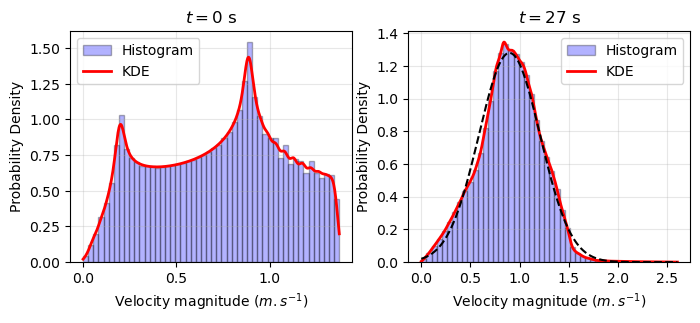
\includegraphics[width=0.5\textwidth]{fig/magnitude_pdf.png}
\caption{Histogram and KDE of velocity magnitude at the start and end of the simulation.}
\label{fig:mag PDF}
\end{figure}

We also examined the angular distribution of the velocity vector relative to the vertical direction (see Figure \ref{fig:angle PDF}). The results show a significant anisotropy developing over time. Initially, energy is injected with a predominantly horizontal forcing, but as the simulation progresses, the vertical direction becomes more dominant, indicating a shift in the orientation of the velocity field.

\begin{figure}[h]
\centering
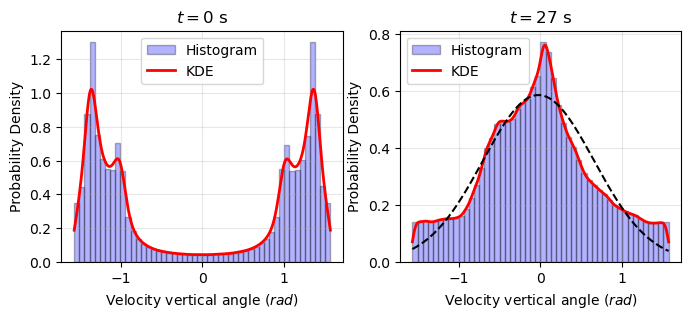
\includegraphics[width=0.5\textwidth]{fig/angle_pdf.png}
\caption{Histogram and KDE of the velocity angle relative to the vertical direction at the start and end of the simulation.}
\label{fig:angle PDF}
\end{figure}

To complement the velocity distribution analysis, we included kernel density estimation (KDE) alongside the histograms. KDE provides a smoothed, continuous representation of the data, offering a clearer view of the distribution compared to the discrete nature of histograms.

\subsection{Energy Spectra}

During the simulation, various spectral quantities are recorded, allowing us to analyze both 1D and 3D energy spectra. Figure \ref{fig:3d spectra time} shows the temporal evolution of the 3D energy spectra, highlighting the development of anisotropy. The energy in the vertical direction surpasses that in the two horizontal directions, with values approximately twice as high: around $0.0024$ compared to $0.001$. After about 5 seconds, the energy distribution stabilizes, indicating that the energy budget no longer evolves significantly over time.

\begin{figure}[h]
\centering
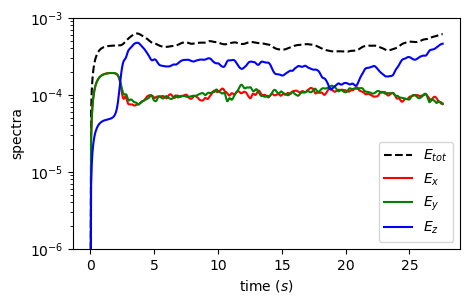
\includegraphics[width=0.5\textwidth]{fig/3d_spectra_time.png}
\caption{Temporal evolution of 3D energy spectra.}
\label{fig:3d spectra time}
\end{figure}

Next, we examine the energy budget as a function of the wave-vector magnitude $k$ by plotting the 1D energy spectra, as shown in Figure \ref{fig:1d spectra}.

\begin{figure}[h]
\centering
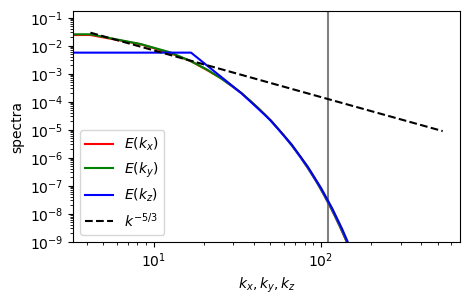
\includegraphics[width=0.5\textwidth]{fig/1d_spectra.png}
\caption{One-dimensional energy spectra. The vertical line indicates the dissipation length scale.}
\label{fig:1d spectra}
\end{figure}

The 1D spectra reveal a clear energy cascade from large to small scales, consistent with the turbulence theory of Kolmogorov [\cite{kolmogorov_local_1941}]. In particular, the energy spectrum follows the expected power-law behavior, $E_k \propto k^{-5/3}$, over the inertial range at the start of the cascade.

\subsection{Richardson Number}

Inspired by the work of \cite{brethouwer_scaling_2007}, we analyze the probability density function (PDF) of the Richardson number throughout the simulation, as shown in Figure \ref{fig:Ri PDF}.

\begin{figure}[h]
\centering
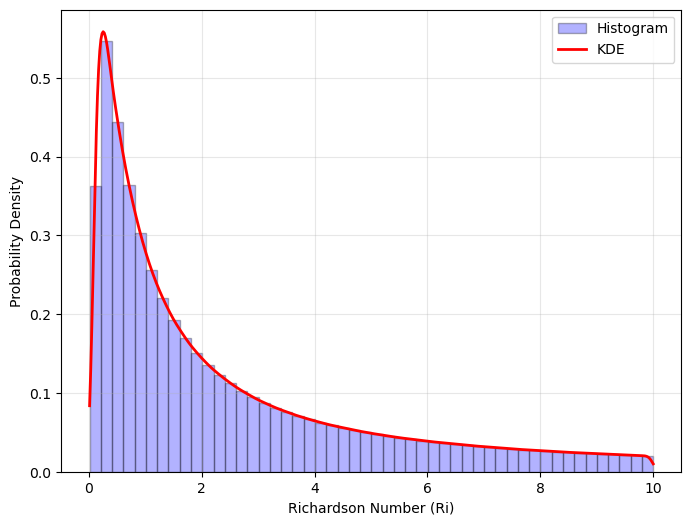
\includegraphics[width=0.5\textwidth]{fig/richardson_pdf.png}
\caption{Histogram and KDE of Richardson number.}
\label{fig:Ri PDF}
\end{figure}

The resulting PDF closely resembles the findings of \cite{brethouwer_scaling_2007}, with a significant concentration of Richardson number values at the lower end of the distribution. This suggests that the flow dynamics share similar characteristics, reinforcing the consistency of the simulated results with prior studies.


\section{Discussion}

As part of a master’s project, this study has focused on simulating stratified turbulence under controlled conditions, providing a foundation for understanding key dynamics. While the results highlight the expected anisotropy and energy cascade in stratified flows, the scope was limited by computational resources and simulation duration. 

Future work could extend this study by exploring a broader range of Richardson numbers, Brunt-Väisälä frequencies, or incorporating rotational effects to simulate more realistic geophysical scenarios. Improving parallelization on HPC clusters would also enable higher-resolution simulations, allowing for more detailed analysis of small-scale dynamics and wave-turbulence interactions.

\section{Summary and conclusions}

\bibliographystyle{elsarticle-harv} 
\bibliography{references.bib}


\end{document}

\endinput